%%%%%%%%%%%%%%%%%%%%%%%%%%%%%%%%%%%%%%%%%%%%%%%%%%%%%%%%%%%%%%%
\section{Preliminaries}\label{sec:preliminaries}

%%%%%%%%%%%%%%%%%%%%%%%%%%%%%%%%%%%%%%%%%%%%%%%%%%%%%%%%%%%%%%%
\subsection{Notation}

% Whenever possible, we denote quantities with upper-case letters and denote either polynomials' degree with lower-case letters.

We denote by $\FF$ to a finite field of prime order $p$ and $\FF^*$ to its respective multiplicative group and define $k$ to be the biggest non-negative integer such that $2^k \mid (p-1)$. We also write $\KK$ to denote a finite field extension of $\FF$, of size $p^e$, $e \geq 2$. 
%where $\phi$ is a root of an irreducible polynomial of the appropriate degree. 
% Given an element $z \in \KK$, we denote the conjugate of $z$ by $\z$. 
% In the context of the Goldilocks prime field, we choose $e=3$ as it is sufficient to achieve sound protocols with state-of-the-art security bounds.
Furthermore, we write $\FF[X]$ (resp. $\KK[X]$) for the ring of polynomials with coefficients over $\FF$ (resp. $\KK$) and write $\FF_{<d}[X]$ (resp. $\KK_{<d}[X]$) to denote the set of polynomials of degree lower than $d$.

Although all the protocols presented in this article work over any prime order, we fix our attention on fields that contain a multiplicative subgroup of size a large power of two. This restriction is crucial to achieving a practical protocol.

% Namely, the prime\footnote{This prime is often incorrectly called a \textit{Goldilocks prime}.} $p = 2^{64} - 2^{32}+1$ is often used not only because it contains a large power of two order multiplicative subgroup, but also because the arithmetic is fast.

Given a cyclic subgroup $S$ of $\FF^*$, we denote by $L_i \in \FF_{<|S|}[X]$ the $i$-th \textit{Lagrange polynomial} for $S$. That is, $L_i$ satisfies $L_i(g^i) = 1$ and $L_i(g^j) = 0$ for $j \neq i$, where $g$ is used here to denote the generator of $S$. Moreover, we denote by $Z_S(X) = X^{|S|} - 1 \in \FF[X]$ to the polynomial that vanishes only over $S$ and call it the \textit{vanishing polynomial} over $S$.
% It can be checked that the $i$-th Lagrange polynomial has the form:
% \[
% L_i(X) = \frac{\omega^i\:(X^n - 1)}{n\:(X - \omega^i)}.
% \]

We denote by $G$ to a cyclic subgroup of $\FF^*$ with order $n$ satisfying $n \mid 2^k$ and $1 < n < 2^k$, and let $g \in \FF$ denote the generator of $G$. Similarly, we denote by $H$ to a nontrivial coset of a cyclic subgroup of $\FF^*$ with order $m$ satisfying $m \mid 2^k$ and $n < m$.

Given a set of polynomials $p_1,p_2,\dots,p_N \in \KK[X]$ we denote by $\MTR(p_1,\dots,p_N)$ to the Merkle root obtained after computing a Merkle tree \cite{C:Merkle87} whose leaves are the evaluations of $p_1,\dots,p_N$ over the domain $H$. Additionally, given a set of elements $x_1,x_2,\dots,x_N \in \KK$, we also use $\MTP(x_1,\dots,x_N)$ to denote the Merkle tree path (i.e., the Merkle proof) computed from the leaf containing these elements. If $X = \{x_1,\dots,x_N\}$, then we use $\MTP(X)$ as a shorthand for $\MTP(x_1,\dots,x_N)$.

Finally, in the description of the protocols, we use $\P$ to denote the prover entity and $\V$ to denote the verifier entity.


%%%%%%%%%%%%%%%%%%%%%%%%%%%%%%%%%%%%%%%%%%%%%%%%%%%%%%%%%%%%%%%
\subsection{Interactive Oracle Proofs and STARKs}\label{sec:IOP}


In this section, we define a polynomial IOP \cite{EPRINT:BenChiSpo16} and the standard security notions associated with this model. Moreover, we introduce a popular polynomial IOP family of protocols known as STIK \cite{C:BBHR19} and explain how a STIK can be compiled into a STARK.

\begin{definition}[Polynomial IOP]
  Given a function $F$, a public coin \textit{polynomial interactive oracle proof (IOP)} for $F$ is an interactive protocol between two parties, the prover $\P$ and the verifier $\V$, that comprises $k$ rounds of interaction. $\P$ is given an input $w$ and both $\P$ and $\V$ are given a common input $x$. At the start of the protocol, $\P$ provides to $\V$ a value $y$ and claims to him the existence of a $w$ satisfying $y = F(x,w)$. 
  
  In the $i$-th round, $\V$ sends a uniformly and independently random message $\alpha_i$ to $\P$. Then $\P$ replies with a message of one of the two following forms: (1) a string $m_i$ that $\V$ reads in full, or (2) an oracle to a polynomial $f_i$ that $\V$ can query (via random access) after the $i$-th round of interaction. At the end of the protocol, $\V$ outputs either $\accept$ or $\reject$, indicating whether $\V$ accepts $\P$'s claim.
\end{definition}

The security notions for IOPs are similar to the security notions of other preceding models (e.g., interactive proofs). In the following definition, probabilities are taken over the internal randomness of $\V$.
\begin{definition}[Completeness and (Knowledge) Soundness]
  We say that a polynomial IOP has \textit{perfect completeness} and \textit{soundness} error at most $\epsilon_s$ if the following two conditions hold. 
  \begin{itemize}
    \item \textbf{Perfect Completeness}. For every $x$ and every prover $\P$ sending a value $y$ satisfying $y = F(x,w)$ at the start of the protocol, it holds that:
    \[
      \Pr\left[\V(x,\P(x,w)) = \accept\right] = 1,
    \]
    where $\V(x,\P(x,w))$ denotes the $\V$'s output after interacting with the prover on input $x$.
    \item \textbf{Soundness}. For every $x$ and every prover $\P^*$ sending a value $y$ at the start of the protocol, if it holds that:
    \[
      \Pr\left[\V(x,\P^*(x,w)) = \accept\right] \geq \epsilon_s,
    \]
    then $y$ satisfies $y = F(x,w)$.
  \end{itemize}
If the next condition holds as well, we say that the polynomial IOP has \textit{knowledge soundness} error at most $\epsilon_{ks}$.
  \begin{itemize}
    \item \textbf{Knowledge Soundness}. There exists a probabilistic polynomial-time algorithm $\E$, known as the \textit{knowledge extractor}, such that for every $x$ and every prover $\P^*$ sending a value $y$ at the start of the protocol if it holds that:
    \[
      \Pr\left[\V(x,\P^*(x,w)) = \accept\right] \geq \epsilon_{ks},
    \]
    then $\E\left(x,\P^*(x,w)\right) = w$ and $y$ satisfies $y = F(x,w)$.
  \end{itemize}
  In words, soundness guarantees that a malicious prover cannot succeed with probability greater than $\epsilon_s$ on the ``existence'' claim of $w$; whereas knowledge soundness guarantees that a malicious prover cannot succeed with probability greater than $\epsilon_{ks}$ claiming ``possession'' of $w$ satisfying $y = F(x,w)$. A polynomial IOP satisfying knowledge soundness is known as a \textit{polynomial IOP of knowledge}.
\end{definition}

Naturally, knowledge soundness implies soundness. Surprisingly, the converse is also true for polynomial IOPs (see, e.g., Lemma 2.3 in \cite{EPRINT:CBBZ22}). This means that proving the soundness of a polynomial IOP is sufficient for achieving knowledge soundness.

% Next, we introduce the definition of a STIK as per Definition 2 in \cite{C:BBHR19}.
\begin{definition}[STIK]
  A \textit{Scalable Transparent polynomial IOP of Knowledge (STIK)} is a polynomial IOP that moreover satisfies the following properties:
  \begin{itemize}
    \item \textbf{Transparent.} They do not require a trusted setup before the execution of the protocol. This setup constitutes a single point of failure and could be exploited by powerful parties to forge false proofs. 
    % In their design, the only cryptographic assumption is the existence of a family of collision-resistant hash functions.  
    \item \textbf{Doubly Scalable.} The verifier runs in time $\O(\log(n))$ and the prover runs in time $\O(n\log(n))$, where $n$ informally denotes the size of the computation $F$.
  \end{itemize}
\end{definition}

When STIKs get instantiated for practical deployment, they result in protocols in which the prover is assumed to be computationally bounded. Protocols of such kind are known as \textit{argument systems} (in contrast to proof systems), and consequently, instantiation of STIKs results in protocols satisfying soundness only against adversaries running in polynomial time.
\begin{definition}[STARK]\label{def:STARK}
  A \textit{scalable transparent argument of knowledge (STARK)} is a realization of a STIK through a family of collision-resistant hash functions. More specifically, polynomial oracles sent from the prover to the verifier in the underlying polynomial IOP are substituted by Merkle roots (computed from polynomial evaluations over a set); and whenever the verifier asks queries to a polynomial $f$ at $v$, the prover answers with $f(v)$ together with the Merkle path associated with it. 
\end{definition}

Finally, we briefly explain how to remove the interaction between a specific prover and verifier of protocols and make them publicly verifiable. The Fiat-Shamir heuristic \cite{C:FiaSha86} can be used to compile a STIK into a non-interactive argument of knowledge in the random oracle model by substituting verifier's messages for queries to the random oracle on input the previous prover's messages until that point. The random oracle is modeled in practice by a cryptographic hash function. Specific details on this compilation will be explained in Section \ref{sec:STIK-to-STARK}. Therefore, a realization of a non-interactive STIK is called a \textit{non-interactive STARK} (but we abuse notation and refer to both as STARKs).




%%%%%%%%%%%%%%%%%%%%%%%%%%%%%%%%%%%%%%%%%%%%%%%%%%%%%%%%%%%%%%%
\subsection{FRI}\label{sec:FRI}

\textit{Fast Reed-Solomon Interactive Oracle Proof of Proximity (FRI)} \cite{EPRINT:BCIKS20} is a protocol for proving that a function $f \colon H \to \FF$ is close to a polynomial of low degree $d$. Here, by low degree, we mean that $d \ll |H|$.
% Recall that the order of $H$ is $m$ while the degree bound will be $n$ with $n < m$ and both, $m$ and $n$ being powers of two.
The FRI protocol consists of two phases. In the first phase, known as the \textit{commit phase}, the prover commits to (via Merkle trees) a series of functions generated from $f$ and random elements $v_0,v_1,\dots$ from $\KK$ provided by the verifier at each round.
Then, in the second phase, known as the \textit{query phase}, the prover provides a set of evaluations of the previously committed functions at a point randomly chosen by the verifier. 
% A sufficiently large repetition of the query phase guarantees the soundness of FRI.
Following, we provide more details about how each phase works.

% \begin{figure}[H]
%   \centering
%   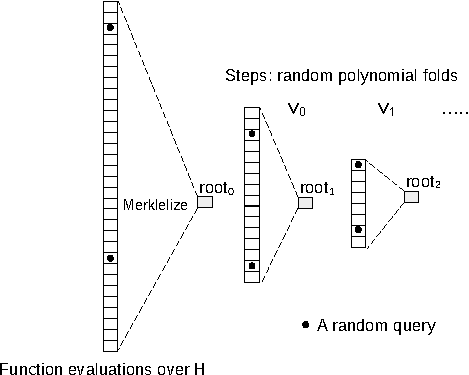
\includegraphics[width=.5\columnwidth]{figures/fri-idea}
%   \caption{Basic FRI Scheme} \label{figure:fri-scheme}
% \end{figure}


%%%%%%%%%%%%%%%%%%%%%%%%%%%%%%%%%%%%%%%%%%%%%%%%%%%%%%%%%%%%%%%
\subsubsection*{The Commit Phase}

Let's denote by $p_0$ the function $f$ of interest and assume for the simplicity of the exposition that the prover is honest (i.e., $p_0$ is a polynomial of low degree).
In the commit phase, the polynomial $p_0$ is split into two other polynomials $g_{0, 1}, g_{0, 2} \colon H^2 \to \KK$ of degree lower than $d/2$. These two polynomials satisfy the following relation with $p_0$:
\begin{equation}\label{eq:FRI-relation}
p_0(X) = g_{0, 1}(X^2) + X \cdot g_{0, 2}(X^2).
\end{equation}

Then, the verifier sends to the prover a uniformly sampled $v_0 \in \KK$, and asks the prover to commit to the polynomial:
\[
p_1(X) := g_{0, 1}(X) + v_0 \cdot g_{0, 2}(X).
\]
Note that $p_1$ is a polynomial of degree less than $d/2$ and the commitment of $p_1$ is not over $H$ but over $H^2 = \{x^2 \colon x \in H\}$, which is of size $|H|/2$.

The prover then continues by splitting $p_1$ into $g_{1, 1}$ and $g_{1, 2}$ of degree lower than $d/4$, then constructing $p_2$ with a uniformly sampled $v_1 \in \KK$ sent by the verifier. Again, $p_2$ is of degree $d/2^2$ and committed over $H^{2^2} = \{x^{2} \colon x \in H^2\}$, whose size is $|H|/2^2$. The whole derivation of $p_{i+1}$ from $p_i$ is often known as \textit{split-and-fold} due to the prover splitting the initial polynomial into two and then folding it into one using a random value. 

The previous process gets repeated a total of $k = \log_2(d)$ times, the point at which $\deg(p_k) = 0$ and the prover sends a constant $p_k$, representing a polynomial of degree lower than $1$, to the verifier.

\begin{figure}[H]
\mypbnonum{}{
  \P(p_0,d,G,H,\FF,\KK) \< \< \V(d,G,H,\FF,\KK) \\[][\hline]
  \< \sendmessageright{top={$\MTR(p_0)$}} \< \\[-2mm]
  \< \sendmessageleft{top={$v_0$}} \< \\[-2mm]
  \< \sendmessageright{top={$\MTR(p_1)$}} \< \\[-2mm]
  \< \sendmessageleft{top={$v_1$}} \< \\[-2mm]
  \< \t\t\t\t\t\t \vdots \< \\
  \< \sendmessageright{top={$\MTR(p_{k-1})$}} \< \\[-2mm]
  \< \sendmessageleft{top={$v_{k-1}$}} \< \\[-2mm]
  \< \sendmessageright{top={$p_k$}} \<
}
\caption{Skeleton description of FRI's commit phase.}
\end{figure}

%%%%%%%%%%%%%%%%%%%%%%%%%%%%%%%%%%%%%%%%%%%%%%%%%%%%%%%%%%%%%%%
\subsubsection*{The Query Phase}

In the query phase, the verifier sends a uniformly sampled $r \in H$ to the prover and queries the evaluations $p_0(r)$, $p_0(-r)$ and $p_1(r^2)$. From $p_0(r)$ and $p_0(-r)$ the verifier computes $p_1(r^2)$ and checks that the computed value matches with the third value $p_1(r^2)$ provided
by the prover.
To obtain $p_1(r^2)$ from $p_0(r)$ and $p_0(-r)$, the verifier first solves the following system of linear equations for $g_{0,1}(r^2),g_{0,2}(r^2)$:
\begin{align*}
  p_0(r) &= g_{0,1}(r^2) + r \cdot g_{0,2}(r^2), \\
  p_0(-r) &= g_{0,1}(r^2) - r \cdot g_{0,2}(r^2),
\end{align*}
and then computes: 
\begin{align*}
  p_1(r^2) = g_{0,1}(r^2) + v_0 \cdot g_{0,2}(r^2).
\end{align*}

The verifier continues by querying for $p_1(-r^2)$ and $p_2(r^4)$. From $p_1(r^2)$ and $p_1(-r^2)$ computes $p_2(r^4)$ as before and checks that the computed value is consistent with $p_2(r^4)$. Each step locally checks the consistency between each pair $(p_i,p_{i+1})$.
The verifier continues in this way until it reaches the value of the constant $p_k$. The verifier checks that the value sent by the prover is indeed equal to the value that the verifier computed from the queries up until $p_{k-1}$. To fully ensure correctness, the prover must accompany the evaluations that he sends with a claim of their existence (via Merkle tree paths). 

\begin{figure}[H]
\mypbnonum{}{
  \P(p_0,d,G,H,\FF,\KK) \< \< \V(d,G,H,\FF,\KK) \\[][\hline]
  \< \t\t\t\t\t\t\t\t\t~~ \vdots \< \\[-2mm]
  \< \sendmessageright{length=6cm,top={$p_k$}} \< \\[-2mm]
  \< \sendmessageleft{length=6cm,top={$r$}} \< \\[-2mm]
  \< \sendmessageright{length=6cm,top={$\{p_0(r),\dots,p_{k-1}(r^{2^{k-1}})\}$},bottom={$\{\MTP(p_0(r)),\dots,\MTP(p_{k-1}(r^{2^{k-1}}))\}$}} \<  \\
  \< \sendmessageright{length=6cm,top={$\{p_0(-r),\dots,p_{k-1}(-r^{2^{k-1}})\}$},bottom={$\{\MTP(p_0(-r)),\dots,\MTP(p_{k-1}(-r^{2^{k-1}}))\}$}} \<
}
\caption{Skeleton description of one iteration of FRI's query phase.}
\end{figure}
Upon the completion of this process, the verifier has a first confirmation that the polynomials committed in the commit phase $p_0,p_1,\dots,p_k$ are consistent with each other. 

Finally, to achieve the required bounds for the soundness of the protocol, the query phase is repeated multiple times. We give the specific soundness bound of a more generic version of FRI in Theorem \ref{thm:batched-FRI-soundness}. The full skeleton description of FRI can be found in Figure \ref{fig:FRI}.


%%%%%%%%%%%%%%%%%%%%%%%%%%%%%%%%%%%%%%%%%%%%%%%%%%%%%%%%%%%%%%%
\subsection*{The Batched FRI Protocol}

In this version of FRI, the prover wants to prove closeness to low-degree polynomials of a set of functions $f_0$,$f_1$,$\dots$,$f_N \colon H \to \FF$ at once. We could run the FRI protocol for every function $f_i$ in parallel, but there is a more efficient way proposed in Section 8.2 of \cite{EPRINT:BCIKS20}. In the batched FRI protocol, the prover instead applies the FRI protocol directly to a random linear combination of the function $f_i$. More specifically, assuming the prover has committed to functions $f_0,f_1,\dots,f_N$ and the verifier has sent a uniformly sampled value $\epsilon \in \KK$, the prover computes the function:
\begin{equation}\label{eq:batched-FRI}
f(X) := f_0(X) + \sum_{i=1}^N \epsilon^i f_i(X),
\end{equation}
and applies the FRI protocol to it.

\begin{remark}
  In \cite{EPRINT:BCIKS20}, they compute $f$ as $f_0(X) + \sum_{i=1}^N \epsilon_i \cdot f_i(X)$ instead, i.e., they use a random value $\epsilon_i \in \KK$ per function $f_i$ instead of powers of a single one $\epsilon$. Even if secure, the soundness bound of this alternative version is linearly increased by the number of functions $N$, so we might assume from now on that $N$ is sublinear in $|\KK|$ to ensure the security of protocols.
\end{remark}

%%%%%%%%%%%%%%%%%%%%%%%%%%%%%%%%%%%%%%%%%%%%%%%%%%%%%%%%%%%%%%%
\subsubsection*{The Batched Consistency Check}

As an extra check in the batched version, the verifier needs to ensure the correct relationship between functions $f_0,\dots,f_N$ and the first FRI polynomial $p_0 = f$. The verifier will use the evaluations of $p_0$ it received from the prover in each FRI query phase invocation. To allow for this check, the prover also sends the evaluations of functions $f_0,f_1,\dots,f_N$ at both $r$ and $-r$ so that the verifier can check that:
\begin{align*}
  p_0(r) &= f_0(r) + \sum_{i=1}^N \epsilon^i f_i(r), \\
  p_0(-r) &= f_0(-r) + \sum_{i=1}^N \epsilon^i f_i(-r),
\end{align*}
i.e., a local consistency check between $f_0,\dots,f_N$ and $p_0$. The prover accompanies the newly sent evaluations with their respective Merkle tree path. The full skeleton description of batched FRI can be found in Figure \ref{fig:batched-FRI}.
% \mypbnonum{}{
%   \P \< \< \V \\[][\hline]
%   \< \t\t\t\t\t\t\t\t\t~~ \vdots \< \\
%   \< \sendmessageright{length=6cm,top={$p_k$}} \< \\[-2mm]
%   \< \sendmessageleft{length=6cm,top={$r$}} \< \\[-2mm]
%   \< \sendmessageright{length=6cm,top={$\{p_0(r),\dots,p_{k-1}(r^{2^{k-1}})\}$},bottom={$\{\MTP(p_0(r)),\dots,\MTP(p_{k-1}(r^{2^{k-1}}))\}$}} \<  \\
%   \< \sendmessageright{length=6cm,top={$\{p_0(r),\dots,p_{k-1}(-r^{2^{k-1}})\}$},bottom={$\{\MTP(p_0(-r)),\dots,\MTP(p_{k-1}(-r^{2^{k-1}}))\}$}} \< \\
%   \< \sendmessageright{length=6cm,top={$\{f_0(r),f_1(r),\dots,f_N(r)\}$},bottom={$\{\MTP(f_0(r)),\dots,\MTP(f_N(r))\}$}} \< \\
%   \< \sendmessageright{length=6cm,top={$\{f_0(-r),f_1(-r),\dots,f_N(-r)\}$},bottom={$\{\MTP(f_0(-r)),\dots,\MTP(f_N(-r))\}$}} \<
% }

Similarly to the non-batched FRI protocol, both the query phase and the batched consistency check gets repeated multiple times to ensure the protocol is sound. More precisely, the soundness error is shown in the following theorem, which is a (somewhat informally) adaptation of Theorems 7.2,8.3 from \cite{EPRINT:BCIKS20}.
\begin{theorem}[Batched FRI Soundness]\label{thm:batched-FRI-soundness}
  Let $f_0,f_1,\dots,f_N$ be functions defined over $H$ and let $m \geq 3$ be an integer. Suppose a batched FRI prover that interacts with a batched FRI verifier causes it to accept with probability greater than:
  \[
    \eFRI = \eC + \eQ^s =  \left( N \cdot \frac{(m + \frac{1}{2})^7}{3 \rho^{3/2}} \cdot \frac{|H|^2}{|\KK|} + N \cdot \frac{(2m+1) \cdot (|H|+1)}{\sqrt{\rho}} \cdot \frac{\sum_{i=0}^{k-1} a_i}{|\KK|} \right) + \left(\sqrt{\rho} \left(1 + \frac{1}{2m}\right)\right)^s,
  \] 
  where $a_i = |H^{2^i}|/|H^{2^{i+1}}|$ is the ratio\footnote{In our case, $a_i = 2$ for all $i$. We decide to not explicitly write it to capture a version of FRI in which some layers of the commit phase can be skipped.} between consecutive prover messages in the commit phase, $\rho = |G| / |H|$ is the rate of the code, $\eC$ and $\eQ$ are respectively the soundness error for the commit and the query phases and $s$ is the number of repetitions of the query phase.

  Then, functions $f_0,f_1,\dots,f_N$ are close to polynomials of degree lower than $n$.
\end{theorem}

%TODO: Check it please! We are not restricting ourselves to Goldilocks now
%TODO: Choose a proper example!
% \begin{example}
%   Say we have $p = 2^{64}-2^{32}+1$, $|\KK| = p^3 \approx 2^{192}$, $|G| = 2^{23}$ and $|H| = 2^{24}$. If we set $m = 3$ and $N = 2^8$, then we have:
%   \[
%     \eC < 2^8 \cdot \frac{2^{14}}{2 \cdot 2^{-3/2}} \cdot \frac{2^{48}}{2^{192}} + 2^8 \cdot \frac{2^{11} \cdot (2^{25})}{2^{-1/2}} \cdot \frac{2^{23}}{2^{192}} < 2^{-120} ,
%   \] 
%   Now, by obtaining $1-\theta = 2^{-1/2} \cdot (1 + \frac{1}{6}) \approx  0.825$ and by setting $s=400$ we have $(1-\theta)^{s} < 2^{-120}$, so the total FRI error is bounded by:
%   \[
%     \eFRI = \eC + (1-\theta)^s < 2^{-120}.
%   \]
% \end{example}
	
In \cite{ICALP:BBHR18} it is shown that for the FRI protocol to achieve security parameter $\lambda$ (i.e., $\eFRI \leq 2^{-\lambda}$), at least $s \geq \lambda/\log_2{\rho^{-1}}$ many queries are needed, and Theorem \ref{thm:batched-FRI-soundness} shows that if $|\KK| \gg |H|^2$ then $s \approx 2\lambda/\log_2{\rho^{-1}}$. 

\begin{figure}[H]
\centering
\hspace{-4.2cm}
\begin{subfigure}[T]{0.4\textwidth}
\mypbnonum{}{
  \P(p_0,\pparams) \< \< \V(\pparams) \\[][\hline]
  \< \sendmessageright{length=6cm,top={$\MTR(p_0)$}} \< \\[-2mm]
  \< \sendmessageleft{length=6cm,top={$v_0$}} \< \\[-2mm]
  \< \sendmessageright{length=6cm,top={$\MTR(p_1)$}} \< \\[-2mm]
  \< \sendmessageleft{length=6cm,top={$v_1$}} \< \\[-2mm]
  \< \t\t\t\t\t\t\t\t\t~~ \vdots \< \\
  \< \sendmessageleft{length=6cm,top={$v_{k-1}$}} \< \\[-2mm]
  \< \sendmessageright{length=6cm,top={$p_k$}} \< \\[-2mm]
  \< \sendmessageleft{length=6cm,top={$h_1$}} \< \\[-2mm]
  \< \sendmessageright{length=6cm,top={$\{p_0(h_1),\dots,p_{k-1}(h_1^{2^{k-1}})\}$},bottom={$\{\MTP(p_0(h_1)),\dots,\MTP(p_{k-1}(h_1^{2^{k-1}}))\}$}} \<  \\
  \< \sendmessageright{length=6cm,top={$\{p_0(-h_1),\dots,p_{k-1}(-h_1^{2^{k-1}})\}$},bottom={$\{\MTP(p_0(-h_1)),\dots,\MTP(p_{k-1}(-h_1^{2^{k-1}}))\}$}} \< \\
  \< \t\t\t\t\t\t\t\t\t~~ \vdots \< \\
  \< \sendmessageleft{length=6cm,top={$h_{s}$}} \< \\[-2mm]
  \< \sendmessageright{length=6cm,top={$\{p_0(h_{s}),\dots,p_{k-1}(h_s^{2^{k-1}})\}$},bottom={$\{\MTP(p_0(h_{s})),\dots,\MTP(p_{k-1}(h_s^{2^{k-1}}))\}$}} \<  \\
  \< \sendmessageright{length=6cm,top={$\{p_0(-h_{s}),\dots,p_{k-1}(-h_s^{2^{k-1}})\}$},bottom={$\{\MTP(p_0(-h_{s})),\dots,\MTP(p_{k-1}(-h_s^{2^{k-1}}))\}$}} \<
}
\caption{ }
\label{fig:FRI}
\end{subfigure}
\hspace{3.8cm}
\begin{subfigure}[T]{0.4\textwidth}
\mypbnonum{}{
  \P(\{f_i\}_i,\pparams) \< \< \V(\pparams) \\[][\hline]
  \< \sendmessageright{length=6cm,top={$\MTR(p_0)$}} \< \\[-2mm]
  \< \sendmessageleft{length=6cm,top={$v_0$}} \< \\[-2mm]
  \< \sendmessageright{length=6cm,top={$\MTR(p_1)$}} \< \\[-2mm]
  \< \sendmessageleft{length=6cm,top={$v_1$}} \< \\[-2mm]
  \< \t\t\t\t\t\t\t\t\t~~ \vdots \< \\
  \< \sendmessageleft{length=6cm,top={$v_{k-1}$}} \< \\[-2mm]
  \< \sendmessageright{length=6cm,top={$p_k$}} \< \\[-2mm]
  \< \sendmessageleft{length=6cm,top={$h_1$}} \< \\[-2mm]
  \< \sendmessageright{length=6cm,top={$\{p_0(h_1),\dots,p_{k-1}(h_1^{2^{k-1}})\}$},bottom={$\{\MTP(p_0(h_1)),\dots,\MTP(p_{k-1}(h_1^{2^{k-1}}))\}$}} \<  \\
  \< \sendmessageright{length=6cm,top={$\{p_0(-h_1),\dots,p_{k-1}(-h_1^{2^{k-1}})\}$},bottom={$\{\MTP(p_0(-h_1)),\dots,\MTP(p_{k-1}(-h_1^{2^{k-1}}))\}$}} \< \\
  \< \sendmessageright{length=6cm,top={$\{f_0(h_1),f_1(h_1),\dots,f_N(h_1)\}$},bottom={$\{\MTP(f_0(h_1)),\dots,\MTP(f_N(h_1))\}$}} \< \\
  \< \sendmessageright{length=6cm,top={$\{f_0(-h_1),f_1(-h_1),\dots,f_N(-h_1)\}$},bottom={$\{\MTP(f_0(-h_1)),\dots,\MTP(f_N(-h_1))\}$}} \< \\
  \< \t\t\t\t\t\t\t\t\t~~ \vdots \< \\
  \< \sendmessageleft{length=6cm,top={$h_{s}$}} \< \\[-2mm]
  \< \sendmessageright{length=6cm,top={$\{p_0(h_{s}),\dots,p_{k-1}(h_s^{2^{k-1}})\}$},bottom={$\{\MTP(p_0(h_{s})),\dots,\MTP(p_{k-1}(h_s^{2^{k-1}}))\}$}} \<  \\
  \< \sendmessageright{length=6cm,top={$\{p_0(-h_{s}),\dots,p_{k-1}(-h_s^{2^{k-1}})\}$},bottom={$\{\MTP(p_0(-h_{s})),\dots,\MTP(p_{k-1}(-h_s^{2^{k-1}}))\}$}} \< \\
  \< \sendmessageright{length=6cm,top={$\{f_0(h_{s}),f_1(h_{s}),\dots,f_N(h_{s})\}$},bottom={$\{\MTP(f_0(h_{s})),\dots,\MTP(f_N(h_{s}))\}$}} \< \\
  \< \sendmessageright{length=6cm,top={$\{f_0(-h_{s}),f_1(-h_{s}),\dots,f_N(-h_{s})\}$},bottom={$\{\MTP(f_0(-h_{s})),\dots,\MTP(f_N(-h))\}$}} \<
}
\caption{ }
\label{fig:batched-FRI}
\end{subfigure}
\caption{Skeleton description of FRI and batched FRI, respectively for (a) and (b). Here, $\pparams = (d,H,\FF,\KK)$.}
\label{fig:STARK1}
\end{figure}
\newpage

%%%%%%%%%%%%%%%%%%%%%%%%%%%%%%%%%%%%%%%%%%%%%%%%%%%%%%%%%%%%%%%
\subsection*{FRI as a Polynomial Commitment Scheme}

Although FRI has a different setting, it can be converted to a \textit{Polynomial Commitment Scheme (PCS)} (for a definition, see \cite{AC:KatZavGol10}) without much overhead. The scheme is based on the following claim: if $f \in \FF[X]$ is a polynomial of degree lower than $d$, then $f(z)$ is the evaluation of $f$ at the point $z$ if and only if $f(X) - f(z) = (X - z) \cdot q(X)$, where $q \in \FF[X]$ is some polynomial of degree lower than $d-1$. 

FRI can be converted to a polynomial commitment scheme as follows. 
\begin{protocol}[FRI-based PCS]
The protocol starts with a function $f \colon H \to \FF$ in possession of the prover. The verifier knows an upper bound $d$ on the degree of $f$.
\begin{enumerate}
  \item As with FRI, the prover's first message is a commitment to $f$. 
  \item The verifier uniformly samples a challenging point $z \in \KK \backslash H$ at which he asks the prover to compute and send the evaluation of $f$.
  \item The prover outputs $f(z)$ along with a FRI proof $\pi_{\text{FRI}}$ that:
  \[
    q(X) := \frac{f(X) - f(z)}{X - z},
  \]
  is close to a polynomial of degree lower than $d-1$.
  \begin{figure}[H]
  \mypbnonum{}{
    \P(f,d,G,H,\FF,\KK) \< \< \V(d,G,H,\FF,\KK) \\[][\hline]
    \< \sendmessageright{length=2cm,top={$\MTR(f)$}} \< \\[-2mm]
    \< \sendmessageleft{length=2cm,top={$z$}} \< \\[-2mm]
    \< \sendmessageright{length=2cm,top={$f(z),\pi_{\text{FRI}}$}} \<
  }
  \caption{Skeleton description of FRI-based PCS.}
  \end{figure}
\end{enumerate} 
If FRI passes, the verifier is convinced with high probability that the prover committed, in the first step, to a polynomial $f$ of degree lower than $d$ and that $f(z)$ is the evaluation of $f$ at $z$.
\end{protocol}

In \cite{EPRINT:VlaPan19}, the authors prove that this scheme satisfies the standard notions of security related to polynomial commitment schemes: correctness, polynomial binding and evaluation binding.


% A proof of the completeness and the soundness of this commitment scheme can be found in  \cite{EPRINT:Habock22}. There, at the same time, it is discussed the need to raise the degree of $q(X)$ multiplying with a degree correction term $1 + \afr X$, being $\afr$ chosen at random by the verifier. This is proposed as a first construction using FRI as a polynomial commitment in order to avoid the case when the prover commits to a degree $n-1$ polynomial $q^*(X)$ whose $f^*(X)$ satisfying
% \[
% q^*(X) \cdot (X - z) = f^*(X) - f(z)
% \] 
% is actually a degree $n$ polynomial. There it is shown that this degree adjustment is, in fact, not necessary. 

%%%%%%%%%%%%%%%%%%%%%%%%%%%%%%%%%%%%%%%%%%%%%%%%%%%%%%%%%%%%%%%
\subsection{Vanilla STARK}\label{sec:vanilla-STARK}

In this section, we review the STARK generation procedure from \cite{EPRINT:StarkWare21} as applied to a particular statement.
%%%%%%%%%%%%%%%%%%%%%%%%%%%%%%%%%%%%%%%%%%%%%%%%%%%%%%%%%%%%%%%
\subsubsection*{Constraints and Trace}

Fix vectors $a,b,c,d,e$ in $\FF^n$. Denote the elements of $a,b,c,d,e$ by $a_i,b_i,c_i,d_i,e_i$, for $i \in [n]$, respectively. Let's say we want to generate a STARK for the following statement: \\[0.2cm]
\fbox{%
\parbox{\textwidth}{
\begin{center}
``I know some $a_i,b_i,c_i,d_i,e_i \in \FF$ such that:
\begin{align}\label{eq:original}
\begin{split}
a_i b_i c_i  &=  a_i + b_i + c_i, \\[0.2cm]
d_i^2 + &2a_{i+1}  =  e_i,
\end{split}
\end{align}
for all $i \in [n]$.''
\end{center}
}%
} \\[0.2cm]

Denote by $\tr_1,\tr_2,\tr_3,\tr_4,\tr_5 \in \FF_{<n}[X]$ the polynomials that interpolate the values $a_i$,$b_i$,$c_i$,$d_i$,$e_i$ over the domain $G$, respectively. That is, $\tr_1(g^i) = a_i$, $\tr_2(g^i) = b_i$, $\tr_3(g^i) = c_i$, $\tr_4(g^i) = d_i$, $\tr_5(g^i) = e_i$ for $i \in [n]$. From now on, we will refer to $G$ as the \textit{trace evaluation domain} and to $\tr_1,\tr_2,\tr_3,\tr_4,\tr_5$ as the \textit{trace column polynomials}.
Hence, the above constraint system (of size $2n$) can be ``compressed'' down into two polynomial constraints through the trace column polynomials. In particular, if for all $x \in G$ the following constraints are true:
\begin{align}\label{eq:constraints}
\begin{array}{ccc}
\tr_1(x) \cdot \tr_2(x) \cdot \tr_3(x) & = & \tr_1(x) + \tr_2(x) + \tr_3(x), \\[0.2cm]
\tr_4(x)^2 + 2 \cdot \tr_1(gx) & = & \tr_5(x),
\end{array}
\end{align}
then the original constraint system \eqref{eq:original} must hold. The prover sends commitments to $\tr_1,\tr_2,\tr_3,\tr_4,\tr_5$ to the verifier.


In general, we will be in the situation of generating a STARK for the knowledge of some polynomials $\tr_1, \dots, \tr_N: G \to \FF$ that satisfy a system of polynomial constraints $\C = \{C_1, \dots, C_\ell \}$, where:
\begin{enumerate}
  \item[(a)] $C_i \in \FF[X_1, \dots, X_N, X'_1, \dots, X'_N]$ for all $i \in [\ell]$.
  \item[(b)] For all $x \in G$ and all $i \in [\ell]$, we have:
  \begin{equation}\label{eq:generic-constraints}
  C_i(\tr_1(x), \dots, \tr_N(x), \tr_1(gx), \dots, \tr_N(gx)) = 0,
  \end{equation}
  when variables $X_j$ are replaced by polynomials $tr_j(X)$ and variables $X'_j$ are replaced by polynomials $tr_j(gX)$ in each $C_i$.
\end{enumerate}
% Observe also that we can view each $\tr_i(X)$ as a polynomial of degree strictly less than $n$. 


%%%%%%%%%%%%%%%%%%%%%%%%%%%%%%%%%%%%%%%%%%%%%%%%%%%%%%%%%%%%%%%
\subsubsection*{From Polynomial Constraints to Rational Functions}\label{sec:constraint-rational}

Given a constraint $C_i$, a rational function is associated with each one of them:
\begin{equation}\label{eq:rational-function}
q_i(X) := \frac{C_i(\tr_1(X), \dots, \tr_N(X), \tr_1(gX), \dots, \tr_N(gX))}{Z_G(X)},
\end{equation}
where, recalling that $\deg(\tr_i) \leq n-1$, each $q_i$ is a polynomial of degree at most $\deg(C_i) \cdot (n - 1) - n$ if and only if the polynomial $Z_G$ divides $C_i$ (i.e., $C_i$ is satisfed over $G$).

Following with our particular example, we have:
\begin{align*}
\begin{array}{rl}
q_1(X) := &\displaystyle \frac{\tr_1(X) \cdot \tr_2(X) \cdot \tr_3(X) - \tr_1(X) - \tr_2(X) - \tr_3(X)}{Z_{G}(X)}, \\[0.4cm]
q_2(X) := &\displaystyle \frac{\tr_4(X)^2 + 2 \cdot \tr_1(gX) - \tr_5(X)}{Z_G(X)},
\end{array}
\end{align*}
where $\deg(C_1)=3$, $\deg(C_2)=2$ and, $q_1(X)$, $q_2(X)$ are of degree at most $2n-3$ and $n-2$, respectively.
% $\deg(a) + \deg(b) + \deg(c) - \deg(Z_G) = 3n-3-n = 2n-3$.
% $2\deg(d) - \deg(Z_G) = 2n-2-n = n-2$.
In fact, the constraints in expression \eqref{eq:constraints} get satisfied if and only if $\deg(q_1) \leq 2n - 3$ and $\deg(q_2) \leq n - 2$. 



%%%%%%%%%%%%%%%%%%%%%%%%%%%%%%%%%%%%%%%%%%%%%%%%%%%%%%%%%%%%%%%
\subsubsection*{The Quotient Polynomial}\label{sec:constraint-polynomial}

In the next step, polynomials $q_i$ are combined into a single polynomial $Q$ known as the \textit{quotient polynomial}. In the STARK proposed in \cite{EPRINT:StarkWare21}, to generate $Q$, the degree of each $q_i$ is adjusted to a sufficiently large power of two.
%We will denote as $\hat{q}_i(X)$ to the corresponding adjusted polynomials.
More precisely, we define $D_i := \deg(C_i)(n-1) - |G|$ and call $D$ to the first power of two for which $D > D_i$ for all $i \in [\ell]$. 
Then, we compute the adjusted version of the rational functions:
\begin{equation}\label{eq:adjusted}
\hat{q}_i(X) := (\afr_iX^{D-D_i-1} + \bfr_i) \cdot q_i(X)
\end{equation}
where $\afr_i, \bfr_i \in \KK$ for all $i\in[\ell]$.

In our example, we have $D_1 = 2n-3,D_2=n-2$, and therefore we take $D = 2n$ (recall $n$ is a power of 2) and then: 
\begin{align*}
\begin{array}{rl}
\hat{q}_1(X) := &(\afr_1 X^2 + \bfr_1) \cdot q_1(X) , \\[0.2cm]
\hat{q}_2(X) := &(\afr_2 X^{n+1} + \bfr_2) \cdot q_2(X) ,
\end{array}
\end{align*} 
hence, $\deg(q_1) \leq 2n-3$ and $\deg(q_2) \leq n - 2$ if and only if $\deg(\hat{q}_1),\deg(\hat{q}_2) < 2n$.

Given polynomials $\hat{q}_i$, we can now compute the quotient polynomial as follows:
\begin{equation}\label{eq:quotient-polynomial}
Q(X) := \sum_{i=1}^{\ell} \hat{q}_i(X) = \sum_{i=1}^{\ell} (\afr_iX^{D-D_i-1} \cdot  \bfr_i) \frac{C_i(\tr_1(X), \dots, \tr_N(X), \tr_1(gX), \dots, \tr_N(gX))}{Z_{G}(X)}
\end{equation}
that satisfies $\deg(Q) < D$. 

Then, $Q$ is split into $S := D/n$ polynomials $Q_1,\dots,Q_S \in \KK[X]$ of degree lower than $n$ satisfying:
\begin{equation}\label{eq:trace-quotient-polynomial}
Q(X) = \sum_{i=1}^S X^{i-1} Q_i(X^S)
\end{equation}
Notice that the polynomials $Q_i$ are bounded by the same degree as the trace column polynomials, so we refer to them as the \textit{trace quotient polynomials}. 

Continuing with our example, the quotient polynomial is $Q(X) := \hat{q}_1(X) + \hat{q}_2(X)$ satisfying $\deg(Q) < 2n$. In this case, we represent the quotient polynomial $Q(X)$ as two polynomials $Q_1,Q_2 \in \FF_{<n}[X]$ such that $Q(X) = Q_1(X^2) + X \cdot Q_2(X^2)$.


%%%%%%%%%%%%%%%%%%%%%%%%%%%%%%%%%%%%%%%%%%%%%%%%%%%%%%%%%%%%%%%
\subsubsection*{Trace Low Degree Extension} 

Since the quotient polynomial $Q$ is defined through rational functions $q_i$ that we are going to evaluate, for Cstr. \eqref{eq:rational-function} to be well-defined, we need to ensure that the denominators of these rational functions are never zero. Therefore, from now on, the polynomials will not be evaluated over the trace evaluation domain, but rather over a larger and disjoint domain, which we refer to as the \textit{evaluation domain}.

More specifically, we introduce the evaluation domain to be:
\begin{enumerate}
	\item Larger than $G$, so that the trace column polynomial has enough redundancy to ensure the soundness of the FRI protocol. 
	
	\item Disjoint of $G$, so that Cstr. \eqref{eq:rational-function} is well-defined.
\end{enumerate}

In order to achieve the previous two requirements, we will choose the evaluation domain to be the coset $H$, where remember that $|H| = 2^k \cdot n$, with $k \geq 1$. We will refer to $2^k$ as the \textit{blowup factor}. Therefore, we need to evaluate all the trace column polynomials over the evaluation domain. We refer to the resulting set of polynomial evaluations as the \textit{trace Low Degree Extension (LDE)}.

The trace LDE is computed in two steps:
\begin{enumerate}
	\item We calculate the interpolation polynomial on the trace evaluation domain of each trace column polynomial using the Inverse Fast Fourier Transform (IFFT). 
	\item We evaluate the polynomials that result from the previous step on the evaluation domain using the Fast Fourier Transform (FFT).
\end{enumerate}





%%%%%%%%%%%%%%%%%%%%%%%%%%%%%%%%%%%%%%%%%%%%%%%%%%%%%%%%%%%%%%%
\subsubsection*{Trace Consistency Check}\label{sec:trace-consistency-check}

At this point, the verifier has everything he needs to perform a local consistency check between the trace column polynomials and the trace quotient polynomials, referred to as the \textit{trace consistency check}. Hence, after the prover commits to the trace quotient polynomials, 
the verifier uniformly samples a random $z$ and requests the prover to send the necessary polynomial evaluations on either $z$ or $gz$. 

More specifically, for a given $z \in \KK \backslash (G \cup \bar{H})$ (here, $\bar{H} = \{x \in \KK \mid x^S \in H\}$) uniformly sampled by a verifier, the prover sends back the trace column polynomials evaluations $\tr_i(z), \tr_j(gz)$ and trace quotient polynomials evaluations $Q_k(z^S)$ for $i,j \in N$ and $k \in [S]$. Notice that the necessary evaluations of the trace column polynomials strictly depend on the particular polynomial expressions in \eqref{eq:generic-constraints}. Denote by $\Evals(z)$ the set of polynomial evaluations over $z$ and by $\Evals(gz)$ the set of polynomial evaluations over $gz$. Naturally, there could exist evaluations of a single polynomial in both sets.

With these evaluations, the verifier can check that:
\begin{align}\label{eq:local-check}
\sum_{i=1}^S z^{i-1} Q_i(z^S) = \sum_{i=1}^\ell (\afr_iX^{D-D_i-1} \cdot  \bfr_i)\frac{C_i(\tr_1(z), \dots, \tr_N(z), \tr_1(gz), \dots, \tr_N(gz))}{Z_G(z)}.
\end{align}

In our particular example, the prover sends back $\tr_1(z)$,$\tr_1(gz)$,$\tr_2(z)$,$\tr_3(z)$,$\tr_4(z)$,$\tr_5(z)$ (so that $\Evals(z) = \{\tr_1(z),\tr_2(z),\tr_3(z),\tr_4(z),\tr_5(z)\}$ and $\Evals(gz) = \{\tr_1(gz)\}$) and $Q_1(z^2),Q_2(z^2)$, and the verifier checks that:
\begin{align}
\begin{array}{cc}
Q_1(z^2) + z \cdot Q_2(z^2) = &~ \displaystyle (\afr_1 z^2 + \bfr_1) \cdot \frac{\tr_1(z) \cdot \tr_2(z) \cdot \tr_3(z) - \tr_1(z) - \tr_2(z) - \tr_3(z)}{Z_G(z)} + \\[0.4cm]
&+ \displaystyle (\afr_2 z^{n+1} + \bfr_2) \cdot \frac{\tr_4(z)^2 + 2\cdot \tr_1(gz) - \tr_5(z)}{Z_G(z)}. 
\end{array}
\end{align}
The problem is that the verifier cannot be sure that the received values are actually the evaluations of previously committed polynomials. In fact, it is easy to obtain values from $\KK$ that satisfy \eqref{eq:local-check} but are not from the expected polynomials. Therefore, after the prover sends the evaluations to the verifier, they engage in the part of the protocol to ensure that the values are the actual evaluations of the corresponding polynomials.  




%%%%%%%%%%%%%%%%%%%%%%%%%%%%%%%%%%%%%%%%%%%%%%%%%%%%%%%%%%%%%%%
\subsubsection*{The FRI Polynomial}

To ensure the validity of the values sent from the prover to the verifier, the prover proceeds to create another set of constraints, then translate them to a problem of low-degree testing, and finally, combines them through the use of random field elements. To this end, the prover computes the $\FRI$ polynomial:
\begin{align}\label{eq:FRI}
\begin{array}{rl}
\FRI(X) := &\displaystyle~\sum_{i \in I_1} \epsilon^{(1)}_i \cdot \frac{\tr_i(X) - \tr_i(z)}{X - z} + \sum_{i \in I_2} \epsilon^{(2)}_i \cdot \frac{\tr_i(gX) - \tr_i(gz)}{X - gz} \\[0.2cm]
	&\displaystyle + \sum_{i=1}^S \epsilon^{(3)}_i \cdot \frac{Q_i(X) - Q_i(z^S)}{X - z^S},
\end{array}
\end{align}
where $I_1 = \{i \in [N] \colon \tr_i(z) \in \Evals(z)\}$, $I_2 = \{i \in [N] \colon \tr_i(gz) \in \Evals(gz)\}$ and $\epsilon^{(1)}_i,\epsilon^{(2)}_j,\epsilon^{(3)}_k \in \KK$ for all $i \in I_1,j\in I_2, k\in[S]$.

What we obtain is that the $\FRI$ polynomial is of degree lower than $n-1$ if and only if: (1) both the trace columns polynomials $\tr_i$ and the trace quotient polynomials $Q_i$ are of degree lower than $n$ and (2) all the values sent by the prover in the previous step are evaluations of the corresponding polynomials.

Finishing with our example, the prover computes the \FRI polynomial as:
\begin{align*}
\begin{array}{rl}
  \FRI(X) := &\displaystyle~\epsilon_1^{(1)} \frac{\tr_1(X) - \tr_1(z)}{X-z} + \epsilon_2^{(1)} \cdot \frac{\tr_2(X) - \tr_2(z)}{X-z} + \epsilon_3^{(1)} \cdot \frac{\tr_3(X) - \tr_3(z)}{X-z} \\[0.4cm]
  &\displaystyle + \epsilon_4^{(1)} \cdot \frac{\tr_4(X) - \tr_4(z)}{X-z} + \epsilon_5^{(1)} \cdot \frac{\tr_5(X) - \tr_5(z)}{X-z} + \epsilon_1^{(2)} \cdot \frac{\tr_1(X) - \tr_1(gz)}{X-gz}\\[0.4cm]
  &\displaystyle + \epsilon_1^{(3)} \cdot \frac{Q_1(X) - Q_1(z^2)}{X-z^2} + \epsilon_2^{(3)} \cdot \frac{Q_2(X) - Q_2(z^2)}{X-z^2}.
\end{array}
\end{align*}

% Observe that the therms corresponding to $\tr_2(gX), \tr_3(gX), \tr_4(gX)$ and  $\tr_5(gX)$ do not appear in the sum because none of the constraints defined before contains them. Then, the $\FRI$ polynomial is of degree lower than $n-1$ if and only if:
% \begin{enumerate}
%   \item[(1)] Both the trace columns polynomials $\tr_1,\tr_2,\tr_3,\tr_4,\tr_5$ and the trace quotient polynomials $Q_1,Q_2$ are of degree lower than $n$.
%   \item[(2)] All the values sent by the prover in the previous step are actually evaluations of the corresponding polynomials.
% \end{enumerate}



%%%%%%%%%%%%%%%%%%%%%%%%%%%%%%%%%%%%%%%%%%%%%%%%%%%%%%%%%%%%%%%
% \subsubsection{Verifying the Trace Values}

% There is an extra detail that needs to be covered at this point. In order to verify that the trace is strictly defined over the base field $\FF$, we proceed with the same methodology as with the evaluations.

% Namely, we compute the $\FRI_2$ polynomial:
% \begin{align}\label{eq:DEEP2}
% \begin{array}{rl}
%   \FRI_2(X) = &\displaystyle~\gamma^8 \cdot \frac{a(X) - \overline{a(z)}}{X-\z} + \gamma^9 \cdot \frac{b(X) - \overline{b(z)}}{X-\z} + \gamma^{10} \cdot \frac{c(X) - \overline{c(z)}}{X-\z} \\[0.4cm]
%   &\displaystyle + \gamma^{11} \cdot \frac{d(X) - \overline{d(z)}}{X-\z} + \gamma^{12} \cdot \frac{e(X) - \overline{e(z)}}{X-\z},
% \end{array}
% \end{align}
% and define $\FRI(X) = \FRI_1(X) + \FRI_2(X)$.

% Thus, the final $\FRI$ polynomial is of degree lower than $n-1$ if and only if conditions (1) and (2) from the $\FRI_1$ polynomial are satisfied and (3) the trace column polynomials are defined over the base field $\FF$.


%%%%%%%%%%%%%%%%%%%%%%%%%%%%%%%%%%%%%%%%%%%%%%%%%%%%%%%%%%%%%%%
\subsubsection*{Proof Verification}

To verify the STARK, the verifier performs the following checks:
\begin{enumerate}
  \item[(a)] \textbf{Trace Consistency.} Checks that the trace quotient polynomials $Q_1, \dots, Q_S$ are consistent with the trace column polynomials $\tr_1, \dots, \tr_N$ by means of the evaluations of these polynomials at either $z$, $gz$ or $z^S$. I.e., the verifier checks that Eq. \eqref{eq:local-check} is satisfied. 
  
  \item[(b)] \textbf{Batched FRI Verification.} It runs the batched FRI verification procedure on the polynomial $\FRI$.

  % \item \textbf{FRI Consistency.} Checks that the polynomials involved in the FRI protocol are consistent with each other. 
  % %Specifically, the verifier uses the evaluations $p_i(h_j^{2^i}), p_i(-h_j^{2^i})$ for $i \in [0,r-1]$ and $j \in [s]$ and the corresponding Merkle proofs, constrasting the received paths with the Merkle tree roots provided in the commit phase along the way.
  
  % \item \textbf{Batched Consistency.} The verifier also checks that the $\FRI$ polynomial is consistent with $\tr_1, \dots,\tr_N, Q_1, \dots, Q_S$ by means of the evaluation of these polynomials in each of the queried points $h_j,-h_j$ for each $j \in [s]$. I.e., the verifier checks that Eq. \eqref{eq:FRI} is satisfied.
\end{enumerate}
If either $(a)$ or $(b)$ fails at any point, the verifier aborts and rejects. Otherwise, the verifier accepts.

The full skeleton description of the vanilla STARK protocol can be found in one-shot in Appendix \ref{sec:vanilla-STARK-description}, in which we include the FRI message exchange in Figure \ref{fig:STARK-vanilla}.

%%%%%%%%%%%%%%%%%%%%%%%%%%%%%%%%%%%%%%%%%%%%%%%%%%%%%%%%%%%%%%%
\subsubsection*{Soundness}

We finally recall the soundness error of the vanilla STARK protocol as in Theorem 4 of \cite{EPRINT:StarkWare21}. Recall that $\rho = |G|/|H|$ is the rate of the code. 
\begin{theorem}[Soundness]\label{thm:STARK-soundness}
  Fix integer $m \geq 3$. Suppose a prover that interacts with a verifier in the vanilla STARK protocol causes it to accept with probability two times greater than:
  \begin{equation}\label{eq:STARK-soundness}
    \eSTARK := \ell \left(\frac{1}{|\KK|} + \frac{(D + |G| + S)\cdot \ell}{|\KK|-S|H|-|G|} \right) + \eFRI,
  \end{equation}
  then Eq. \eqref{eq:generic-constraints} is satisfied (i.e., the original statement is true), where $\ell = m/\rho$ and $\eFRI$ is as defined in Theorem \ref{thm:batched-FRI-soundness}.
\end{theorem}
We give some intuitions for the computation of this error bound. The first term in Eq. \eqref{eq:STARK-soundness} corresponds to the probability of sets $\{\afr_1,\bfr_1,\dots,\afr_T,\bfr_T\}$ being ``good'' under a dishonest prover. This means that if all $\afr_i,\bfr_i$ are uniformly and independently randomly sampled, then the probability the quotient polynomial $Q$ is a polynomial is at most $\ell/|\KK|$. The second term corresponds to the probability of sampling a $z \in \KK \backslash (G \cup \bar{H})$ for which the FRI protocol passes with a probability greater than $\eFRI$.


%%%%%%%%%%%%%%%%%%%%%%%%%%%%%%%%%%%%%%%%%%%%%%%%%%%%%%%%%%%%%%%%
\subsection{Arguments}\label{sec:preliminaries:arguments}

In this section, we introduce the ``arguments'' that we will use to extend the vanilla STARK. Here, by argument, we mean a relation between polynomials that cannot be directly expressed through an identity. We often refer to these arguments as \textit{non-identity constraint}. The three arguments we will introduce are \textit{multiset equality}, \textit{connection} and \textit{inclusion}.

The protocols that instantiate these arguments are all based on the same idea of the computation of a grand product polynomial over the two (or more) vectors involved in the argument. Specifically, a polynomial is cumulatively computed as the quotient of a function of the first vector and a function of the second vector. Then, a set of identities is proposed as insurance for a verifier of the protocol that not only the grand product was correctly computed by a prover, but also that the specific intention of the protocol is satisfied. To ensure the soundness of the protocols, random values uniformly sampled by the verifier are used in such computation.

% An alternative to the previous idea is based on the addition of logarithmic derivatives (see e.g. \cite{EPRINT:Habock22b}) instead, but they come with tradeoffs that make them unwanted for the STARK context. 

Recall that $G = \langle g \rangle$ is a cyclic subgroup of $\FF^*$ of order $n$.

%%%%%%%%%%%%%%%%%%%%%%%%%%%%%%%%%%%%%%%%%%%%%%%%%%%%%%%%%%%%%%%%
\subsubsection*{Multiset Equality}

Given two vectors $f = (f_1, \dots, f_n)$ and $t = (t_1, \dots, t_n)$ in $\FF^n$, a multiset equality argument, denoted $f \doteq t$, is used for checking that $f$ is equal to $t$ as multisets (or equivalently, that $f$ and $t$ are a permutation of each other). The protocol that instantiates the multiset equality arguments works by computing the following grand product polynomial $Z \in \KK_{<n}[X]$:
\[
  Z(g^i) = 
  \begin{cases} 
  1, & \text{if }~ i=1 \\ 
  \displaystyle\prod_{j=1}^{i-1} \frac{(f_j + \gamma)}{(t_j + \gamma)}, & \text{if }~ i = 2, \dots, n
  \end{cases} 
\]
where $\gamma \in \KK$ is the value sent from the verifier. 

The definition of the previous polynomial is based on the following lemma.
\begin{lemma}[Soundness of Multiset Equality]\label{lemma:muleq-soundness}
  Fix two vectors $f = (f_1, \dots, f_n)$ and $t = (t_1, \dots, t_n)$ in $\FF^n$. If the following holds with probability larger than $\eMulEq(n) := n/|\KK|$ over a random $\gamma \in \KK$:
  \begin{equation*}
  \prod_{i=1}^n (f_i + \gamma) = \prod_{i=1}^n (t_i + \gamma),
  \end{equation*}
  then $f \doteq t$. 
\end{lemma}
\begin{proof}
  Assume that $f \not\doteq t$. Then, there must be some $i^* \in [n]$ such that $t_{i^*} \neq f_i$ for all $i \in [n]$. Define degree $n$ polynomials $F(X) := \prod_{i=1}^n (f_i + X)$ and $T(X) := \prod_{i=1}^n (t_i + X)$. By the assumption, we have that $F \neq T$ and therefore by the Schwartz-Zippel lemma $F(\gamma) \neq T(\gamma)$ except with probability $n/|\KK|$.
\end{proof}

As a consequence of Lemma \ref{lemma:muleq-soundness}, the identities that must be checked by the verifier for $x \in G$ are the following: 
\begin{align} \label{eq:permutation-Z}
&L_1(x) \cdot (Z(x) - 1) = 0, \\
&Z(x \cdot g) \cdot (t(x) + \gamma) = Z(x) \cdot (f(x) + \gamma),
\end{align}
where $f,t \in \FF_{<n}[X]$ are the polynomials resulting from the interpolation of $\{f_i\}_{i\in[n]}$ and $\{t_i\}_{i\in[n]}$ over $G$,respectively.




%%%%%%%%%%%%%%%%%%%%%%%%%%%%%%%%%%%%%%%%%%%%%%%%%%%%%%%%%%%%%%%%
\subsubsection*{Connection}

The protocol for a connection argument and the definitions and results we provide next are adapted from \cite{EPRINT:GabWilCio19}.

Given some vectors $f_1,\dots,f_k \in \FF^n$ and a partition $\T = \{T_1,\dots,T_s\}$ of the set $[kn]$, a connection argument, denoted $(f_1,\dots,f_k) \propto \{T_1,\dots,T_s\}$, is used to check that the partition $\T$ divides the field elements $\{f_{i,j}\}_{i\in[k],j\in[n]}$ into sets with the same value. More specifically, if we define the sequence $f_{(1)},\dots,f_{(kn)} \in \FF$ by:
\[
  f_{((i-1)n + j)} := f_{i,j}
\]
for each $i \in [k], j \in [n]$, then we have $f_{(\ell_1)} = f_{(\ell_2)}$ if and only if $\ell_1,\ell_2$ belong to the same block of $\T$. 

In order to express the partition $\T$ within a grand product polynomial, we define a permutation $\sigma\colon [kn] \to [kn]$ as follows: $\sigma$ is such that for each block $T_i$ of $\T$, $\sigma(\T)$ contains a cycle going over all elements of $T_i$. Then, the protocol that instantiates the connection arguments works by computing the following grand product polynomial $Z \in \KK_{<n}[X]$:
\[
  Z(g^i) = 
  \begin{cases} 
  1, & \text{if }~ i=1 \\ 
  \displaystyle\prod_{\ell=1}^{k}\prod_{j=1}^{i-1} \frac{(f_{\ell,j} + \gamma \cdot (\ell-1)\cdot n +j) + \delta)}{(f_{\ell,j} + \gamma \cdot \sigma((\ell-1)\cdot n +j) + \delta)}, & \text{if }~ i = 2, \dots, n
  \end{cases} 
\]
where $\gamma,\delta \in \KK$ are the values sent from the verifier. 


The definition of the previous polynomial is based on the following lemma, a proof of which can be found\footnote{The claim in \cite{EPRINT:GabWilCio19} is for a slightly more general protocol.} in Claim A.1. of \cite{EPRINT:GabWilCio19} and is similar to the one of Lemma \ref{lemma:muleq-soundness}.
\begin{lemma}[Soundness of Connection]\label{lemma:connection-soundness}
Fix $f_1,\dots,f_k \in \FF^n$ and a partition $\T = \{T_1,\dots,T_s\}$ of $[kn]$. If the following holds with probability larger than $\eCon(n) := kn/|\KK|$ over randoms $\gamma, \delta \in \KK$:
\[
\prod_{\ell=1}^k \prod_{j=1}^n (f_{\ell,j} + \gamma \cdot ((\ell-1)\cdot n + j) + \delta) = \prod_{\ell=1}^k \prod_{j=1}^n (f_{\ell,j} + \gamma \cdot \sigma((\ell-1)\cdot n + j) + \delta),
\]
then, $(f_1,\dots,f_k) \propto \{T_1,\dots,T_s\}$.
\end{lemma}

As a consequence of Lemma \ref{lemma:connection-soundness}, the identities that must be checked by the verifier for $x \in G$ are the following: 
\begin{align} \label{eq:connection-Z}
\begin{array}{c}
  L_1(x) \cdot (Z(x) - 1) = 0, \\[0.2cm]
  \displaystyle Z(x \cdot g)  = Z(x) \cdot \frac{(f_{1}(x) + \gamma \cdot S_{\ID_1}(x) + \delta)}{(f_{1}(x) + \gamma \cdot S_{\sigma_1}(x) + \delta)} \cdot \cdots \cdot \frac{(f_{k}(x) + \gamma \cdot S_{\ID_k}(x) + \delta)}{(f_{k}(x) + \gamma \cdot S_{\sigma_k}(x) + \delta)},
\end{array}
\end{align}
where $S_{\ID_{i}}(g^j) = (i-1)\cdot n +j$ is the polynomial mapping $G$-elements to indexes in $[kn]$ and $S_{\sigma_{i}}(g^j) = \sigma((i-1)\cdot n +j)$ is the polynomial defined by $\sigma$. Since the permutation $\sigma$ perfectly relates with the partition $\T$ it refers to, from now on we denote a connection argument between polynomials $f_1,\dots,f_k \in \FF[X]$ and a partition $\T$ as $(f_1,\dots,f_k) \propto (S_{\sigma_1},\dots,S_{\sigma_k})$. As we will see in later sections, this overloading notation will become very natural.

For more details see \cite{EPRINT:GabWilCio19}.


%%%%%%%%%%%%%%%%%%%%%%%%%%%%%%%%%%%%%%%%%%%%%%%%%%%%%%%%%%%%%%%%
\subsubsection*{Inclusion}

The protocol for an inclusion argument and the definitions and results we provide next is adapted from the well-known Plookup protocol \cite{EPRINT:GabWil20}, with the ``alternating method''  provided in \cite{EPRINT:PFMBM22}.

Given two vectors $f = (f_1, \dots, f_n)$ and $t = (t_1, \dots, t_n)$ in $\FF^n$, a inclusion argument, denoted $f \in t$, is used for checking that the set $A$ formed with the values $\{f_i\}_{i\in[n]}$ is contained in the set $B$ formed with the values $\{t\}_{i\in[n]}$. Notice that $|A|,|B|\leq n$.

In the protocol, the prover has to construct an auxiliary vector $s = (s_1, \dots, s_{2n})$ containing every element of $f$ and $t$ where the order of appearance is the same as in $t$.
The main idea behind the protocol is that if $f \in t$, then $f$ contributes to $s$ with repeated elements.
To check this fact, a vector $\Delta{s}$ is defined as follows:
\[
\Delta{s} = (s_1+\gamma\,s_2, s_2+\gamma\,s_3, \cdots, s_{2n}+\gamma\,s_1).
\]

Then, the protocol essentially checks that $\Delta{s}$ is consistent with the elements of $f$, $t$ and $s$.
To do so, the vector $s$ is split into two vectors $h_1,h_2 \in \FF^n$.
In the protocol described in \cite{EPRINT:GabWil20},
$h_1$ and $h_2$ contain the lower and upper halves of $s$, while in our protocol in \cite{EPRINT:PFMBM22}, we use $h_1$ to store elements with odd indexes and $h_2$ for even indexes, that is:
\begin{equation}\label{eq:alternating-method}
h_1 = (s_1, s_3, s_5, ..., s_{2n-1}) \quad\text{ and }\quad
h_2 = (s_2, s_4, s_6, ..., s_{2n}).
\end{equation}

With this setting in mind, the grand product polynomial is defined as:
\[
  Z(g^i) = 
  \begin{cases} 
  1, & \text{if }~ i=1 \\ 
  \displaystyle (1+\gamma)^{i-1}\prod_{j=1}^{i-1}\frac{{(\delta + f_j)}   (\delta(1+\gamma) + t_j + \gamma t_{j+1})}{ (\delta(1+\gamma) + s_{2j-1} + \gamma s_{2j})(\delta(1+\gamma) + s_{2j} + \gamma s_{2j+1})}, & \text{if }~ i = 2, \dots, n
  \end{cases} 
\]
where $\gamma,\delta \in \KK$ are the values sent from the verifier.

The definition of the previous polynomial is based on the following lemma, which is a slight modification of Claim 3.1. of \cite{EPRINT:GabWil20}.
\begin{lemma}[Soundness of Inclusion]\label{lemma:inclusion-soundness}
  Fix three vectors $f = (f_1, \dots, f_n),t = (t_1, \dots, t_n)$ and $s = (s_1,\dots,s_{2n})$ with elements in $\FF$. If the following holds with probability larger than $\eInc(n) := (4n-2)/|\KK|$ over randoms $\gamma, \delta \in \KK$:
  \begin{equation*}
    (1+\gamma)^n\prod_{i=1}^n (\delta + f_i)\prod_{i=1}^{n-1} (\delta(1+\gamma) + t_i + \gamma t_{i+1}) = \prod_{i=1}^{2n-1} (\delta(1+\gamma) + s_i + \gamma s_{i+1}),
  \end{equation*}
  then $f \in t$ and $s$ is the sorted by $t$ concatenation of $f$ and $t$. 
\end{lemma}

As a consequence of Lemma \ref{lemma:inclusion-soundness}, the identities that must be checked by the verifier for $x \in G$ are the following: 
\begin{align} \label{eq:look-Z}
\begin{array}{c}
  L_1(x) \left( Z(x) - 1\right) = 0, \\[0.2cm]
  Z(x\cdot g) = \displaystyle Z(x)\frac{(1+\gamma)(\delta + f(x))(\delta(1+\gamma) + t(x) + \gamma t(gx))}{(\delta(1+\gamma) + {h_1}(x) + \gamma {h_2}(x))(\delta(1+\gamma) + {h_2}(x) + \gamma {h_1}(x\cdot g))}.
\end{array}
\end{align}
where $f,t \in \FF_{<n}[X]$ are the polynomials resulting from the interpolation of $\{f_i\}_{i\in[n]}$ and $\{t_i\}_{i\in[n]}$ over $G$, respectively; and $h_1,h_2 \in \FF_{<n}[X]$ are the polynomials resulting from the interpolation of the values defined in Eq. \eqref{eq:alternating-method} over $G$.

For more details see \cite{EPRINT:GabWil20} and \cite{EPRINT:PFMBM22}.
